\chapter[Coalitions et séparation des pouvoirs]{RAW, Eric Temple Bell, la Loi des Cinq, coalitions et séparation des pouvoirs}
\chapterauthor{Griffensteed the 5$^\text{lth}$}

\blockquote{
\small{``Ce que Weishaupt découvrit cette nuit du 2 février, dix-sept soixante-seize," expliqua Hagbard Celine à Joe Malik en 1973, par une claire journée d'automne à Miami, à peu près au même moment où le capitaine Tequilla y Mota lisait Luttwak sur le coup d'État et faisait ses premiers pas vers la cabale de l'officier qui a ensuite saisi Fernando Poo,``était essentiellement une simple relation mathématique. C'est si simple, en fait, que la plupart des administrateurs et des bureaucrates ne le remarquent jamais. convoitise, tel le propriétaire ne remarque pas l'humble termite, jusqu'à ce qu'il soit trop tard. . . . Tiens, prends ce papier et fais-toi une idée. Combien de permutations y a-t-il dans un système à quatre éléments ?

Joe, se souvenant des mathématiques de lycée, écrivit $4\times3\times3\times2\times1\times1$, et lut à haute voix sa réponse ``vingt-quatre''.

``Et si tu es l'un des éléments, le nombre de coalitions --- ou pour être sinistre, de conspirations --- que tu pourrais avoir à affronter serait de vingt-trois. Malgré les obsessions de Simon Moon, le vingt-trois n'a pas de signification mystique particulière," ajouta rapidement Hagbard. ``Il s'agit d'un certain nombre de relations possibles dont le cerveau peut se souvenir et gérer. Mais supposons maintenant que le système comporte cinq éléments . . . ?.''

Joe écrivit 5$\times4\times3\times3\times2\times1$ et lut à haute voix, ``Cent vingt-et-un."

``Tu vois ? On rencontre toujours des sauts de cette taille lorsqu'il s'agit de permutations et de combinaisons. Mais, comme je l'ai dit, en règle générale, les administrateurs n'en sont pas conscients. Korzybski a fait remarquer, au début des années trente, que personne ne devrait jamais superviser directement plus de quatre subordonnés, parce que les vingt-quatre coalitions possibles que la politique de bureau ordinaire peut créer suffisent à taxer n'importe quel cerveau. Quand il saute à cent vingt, l'administrateur est perdu. C'est là, par essence, l'aspect sociologique de la mystérieuse Loi des Cinq. Les Illuminati ont toujours cinq dirigeants dans chaque nation, et cinq Illuminati Primi internationaux qui les supervisent tous, mais chacun dirige son propre spectacle plus ou moins indépendamment des quatre autres, unis seulement par leur engagement commun à l'Objectif du Gruad." Hagbard s'arrêta pour rallumer son long cigare italien noir.}
\par\begin{flushright} \textup{--- Robert Shea \& Robert Anton Wilson}, Illuminatus!, 1975. \end{flushright}
}

\begin{center}

\includegraphics[scale=0.1]{./img/eris.png}
\end{center}

\section*{Combinatoire des coalitions}
Contrairement à ce qu'explique Hagbard Celine dans cet extrait introductif, le nombre de coalitions --- ou, pour être sinistre, de conspirations --- que l'on peut obtenir avec un système de $n$ éléments n'est pas lié au nombre de permutations mais a plutôt rapport avec le problème de partition d'un ensemble ; un autre problème de combinatoire définit par une relation mathématique plus complexe.\\

D'une part, le nombre de permutations de $n$ éléments correspond au nombre de façons de disposer ces $n$ éléments dans une ligne \cite{Graham1988}. Par exemple, pour l'ensemble $\{1,2,3\}$ il y a six permutations possibles :
\begin{gather*}
(1,2,3) \qquad (1,3,2) \qquad (2,1,3) \\ 
(2,3,1) \qquad (3,1,2) \qquad (3,2,1)
\end{gather*}
Dans ce cas, Joe Malik a fait le calcul correct lorsqu'il s'agissait de permutations, en suivant les instructions de Hagbard. Il y a $n$ choix pour le premier élément, $n-1$ pour le deuxième, $n-2$ pour le troisième, et ainsi de suite, donnant $n\times(n-1)\times(n-2)\times(n-2)\times...\times1$, c'est à dire
\begin{equation}
n ! = \prod\limits_{k = 1}^n k
\end{equation}
La séquence entière des nombres factoriels (commençant par $0!$) est : $1, 1, 1, 2, 6, 24, 120, 720, ....$ (séquence A000142 sur l'Encyclopédie en ligne des séquences entières\footnote{\url{https://oeis.org}}).
Cependant, les permutations ne montrent que des façons d'organiser les éléments, mais ne traitent pas des différentes façon de regrouper les éléments et ne sont donc pas un bon modèle pour traiter des coalitions.\\

D'autre part, une partition d'un ensemble $S$ constitué de $n$ éléments est une famille de sous-ensembles de $S$ disjoints appelés ``blocs'' dont l'union est $S$ \cite{Rota1964}.
En d'autres termes, elle correspond à une façon de regrouper tous les éléments de l'ensemble en sous-ensembles, c'est-à-dire les différentes coalitions possibles avec $n$ éléments. Par exemple, pour l'ensemble $\{1,2,3\}$, il y a cinq partitions possibles :
\begin{gather*}
(\{1\},\{2\},\{3\}) \quad (\{1,2\},\{3\}) \quad (\{1,3\},\{2\}) \\
(\{1\},\{2,3\}) \quad  (\{1,2,3\})
\end{gather*}
Compter le nombre de partitions d'un ensemble avec $n$ éléments est un peu plus compliqué. Il correspond au nombre de Bell $B_n$, nommé d'après le mathématicien Eric Temple Bell, et peut être calculé à l'aide de la formule récursive suivante :

\begin{equation}
    \begin{cases}
         B_0 = 1\\
         B_{n+1} = \sum\limits_{k=0}^n \binom nk B_k \quad \text{.}
     \end{cases}
\end{equation}
La démonstration de cette formule et d'autres formules pour les nombres de Bell peut se trouver dans \cite{Graham1988, Rota1964}.
Une autre méthode pour calculer les nombres de Bell consiste à construire le triangle de Bell \cite{Aitken1933}. Ce triangle est construit en suivant les règles suivantes :
\begin{itemize}
\item commencer par le chiffre 1,
\item pour chaque nouvelle ligne, la valeur la plus à gauche est une copie de la valeur la plus à droite de la ligne précédente,
\item toutes les autres valeurs sont la somme de la valeur à sa gauche et de celle en diagonal en haut à gauche.
\end{itemize}
 Les premières rangées du triangle de Bell sont illustrées dans la Figure \ref{bell}. La séquence entière des nombres de Bell (à partir de $B_0$) est : $1, 1, 1, 2, 5, 15, 52, 203, ....$ (séquence A000110 sur l'OEIS).\\

\begin{figure}[h]
\begin{center}
 \[ 
    \begin{matrix}
    1 & & & & & & & \longrightarrow & B_1= 1\\
    1 & 2 & & & & & & \longrightarrow & B_2= 2\\
    2 & 3 & 5 & & & & & \longrightarrow & B_3= 5\\
    5 & 7 & 10 & 15 & & &&  \longrightarrow & B_4= 15\\
    15 & 20 & 27 & 37 & 52 & & & \longrightarrow & B_5= 52\\
    52 & 67 & 87 & 114 & 151 & 203 & & \longrightarrow & B_6= 203\\    
    \vdots\\
    \end{matrix}
\]
\caption{\label{bell} Premières lignes du triangle de Bell.}
\end{center}
\end{figure}

Les choses se compliquent encore plus si l'on considère que les partitions peuvent être ordonnées. Dans ce cas, les différentes permutations d'une partition donnée doivent être prises en compte. C'est ce qu'on appelle un ordonnancement faible et cela peut être utilisé pour déterminer le nombre de façons de classer $n$ joueurs lorsque les \emph{ex-aequo} sont possibles \cite{Good1975}. Dans notre cas, il peut être utilisé pour représenter les relations de pouvoir déséquilibrées entre les différents éléments/coalitions. Par exemple, pour l'ensemble $\{1,2,3\}$, il y a treize \emph{partitions ordonnées} possibles :
\begin{gather*}
(\{1\},\{2\},\{3\}) \quad (\{1\},\{3\},\{2\}) \\ 
(\{2\},\{1\},\{3\}) \quad (\{2\},\{3\},\{1\}) \\ 
(\{3\},\{1\},\{2\}) \quad (\{3\},\{2\},\{1\}) \\
(\{1\},\{2,3\}) \quad (\{2,3\},\{1\}) \quad (\{2\},\{1,3\}) \\
(\{1,3\},\{2\}) \quad (\{3\},\{1,2\}) \quad (\{1,2\},\{3\}) \\
(\{1,2,3\})
\end{gather*}
Le nombre de partitions ordonnées possibles d'un ensemble d'éléments $n$ est donné par les nombres de Bell ordonnés (aussi appelés nombres de Fubini), définis par \cite{Knuth1998} :
\begin{equation}
     a_n= \sum\limits_{k=0}^n k ! S(n,k) \quad \quad \text{,}
\end{equation}
où $S(n,k)$ est le nombre de Stirling de seconde espèce, correspondant au nombre de façons de partitionner un ensemble de $n$ éléments en $k$ sous-ensembles non vides, et peut être calculé avec la formule récursive \cite{Graham1988} :
\begin{equation}
    \begin{cases}
    S(0,0) = 1 \quad \text{and} \quad S(0,n) = S(n,0) = 0\\
    S(n+1,k) = kS(n,k) + S(n,k-1)
    \end{cases}
\end{equation}
La séquence entière des nombres de Bell ordonnés (à partir de $a_0$) est : $1, 1, 1, 3, 13, 75, 541, 4683, ....$ (séquence A000670 sur l'OEIS).

\section*{Les répercussions}

De retour à nos coalitions --- ou pour être sinistre, conspirations --- et à l'extrait d'\textit{Illuminatus!} Si nous considérons d'abord les partitions non ordonnées : ``Combien de partitions différentes y a-t-il dans un système à quatre éléments ?", aurait dû demander Hagbard Céline.\\
Joe écrivit le début de la séquence des nombres de Bell et lut à haute voix ``le quatrième nombre de Bell est quinze."\\
Donc, si on supprime l'état où tous les éléments sont séparés, c'est-à-dire sans coalition, cela signifie que le nombre de coalitions possibles avec quatre éléments auxquels on pourrait avoir à faire serait de quatorze\footnote{$1+4=5$, mais oublions la magick de la Loi des Cinq\cite{Malaclypse1963}.}. Et maintenant, qu'en est-il d'un système à cinq éléments ?\\
Joe lut à haute voix ``le cinquième nombre de Bell est cinquante-deux."\\
De même, le nombre de coalitions possibles avec cinq éléments auxquels on pourrait avoir à faire serait de cinquante et un. La Figure \ref{part} montre les 52 différentes partitions possibles pour un ensemble de 5 éléments.
Dans ce cas, même si le problème n'a pas été correctement résolu par l'utilisation de permutations au lieu de partitions, la déduction de RAW et de Korzybski est toujours valable. 
Le saut de quatorze à cinquante et une relations possibles est suffisant pour passer de quelque chose d'épuisant pour l'esprit à quelque chose d'assez grand pour le perdre complètement \cite{Kelly1955, Korzybski1933}. \\

\begin{figure}
\begin{center}
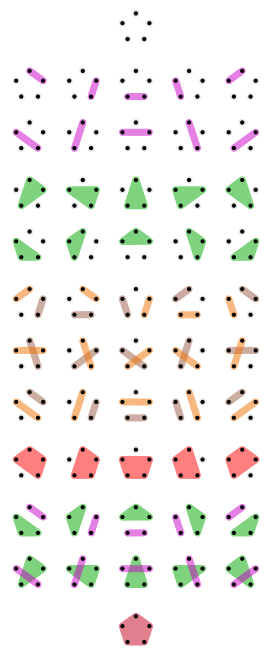
\includegraphics[scale=0.7]{./img/part.png}
\caption{\label{part} Les 52 partitions d'un ensemble à 5 elements (source: wikipedia).}
\end{center}
\end{figure}

Maintenant, si nous considérons les partitions ordonnées, le saut apparaît plus tôt. Le troisième nombre de Fubini est treize et le quatrième nombre de Fubini est soixante-quinze \footnote{$75=5\times 15$ }. De plus, dans ce cas, toutes les configurations sont problématiques, puisqu'elles représentent soit des coalitions, soit des rapports de force déséquilibrés entre les éléments. Avec ce modèle, la déduction de RAW et de Korzybski apparaît plus tôt qu'ils ne l'ont formulé en termes de nombre d'éléments ; quatre éléments devenant le nouveau point de basculement.


\section*{La Loi des Cinq et la séparation des pouvoirs}

Lorsqu'ils expriment les bases nécessaires pour obtenir une véritable démocratie, John Locke et Montesquieu identifient le besoin de séparation des pouvoirs (c'est-à-dire l'absence de coalition entre les pouvoirs) pour les \textit{démocraties représentatives} dans leurs essais respectifs \textit{Traité du gouvernement civil} \cite{Locke1689} et \textit{De l'esprit des lois} \cite{Montesquieu1748}. De plus, les critiques modernes de leurs travaux, lorsqu'il s'agit de l'établissement d'une démocratie, visent d'abord le fait que les organisations proposées respectivement par Locke et Montesquieu n'assurent pas une réelle séparation des pouvoirs mais plutôt une interdépendance des pouvoirs ; puis le fait que les différents pouvoirs identifiés ne sont pas mis sur un pied d'égalité, certains étant plus importants que d'autres.\\

Montesquieu identifie trois pouvoirs \cite{Montesquieu1748}, qui sont maintenant représentés par différentes institutions dans de nombreuses démocraties représentatives à la suite du \textit{Siècle des Lumières} :
\begin{itemize}
\item le pouvoir législatif,
\item le pouvoir exécutif,
\item le pouvoir judiciaire.
\end{itemize}
Dans ce contexte avec trois pouvoirs, le troisième nombre de Bell nous indique que le nombre de coalitions possibles (et donc l'absence de réelle séparation des pouvoirs) est de quatre ($B_3 - 1$), et le troisième nombre de Fubini nous indique que le nombre de coalitions possibles ou de relations de pouvoir déséquilibrées (et donc l'absence de véritable séparation des pouvoirs ou d'égalité entre pouvoirs) est de treize ($a_3$).\\
En d'autres termes, avec les deux modèles, nous obtenons un certain nombre de relations possibles que le cerveau, les institutions et les gens peuvent gérer.
Il serait donc théoriquement possible d'obtenir une véritable démocratie avec une démocratie représentative.\\

Cependant, de nouveaux pouvoirs ont été identifiés depuis. En particulier :
\begin{itemize}
\item le pouvoir médiatique (aussi appelé ``le quatrième pouvoir'') \cite{Bourdieu1996, Herman1988},
\item le pouvoir économique (aussi appelé ``le cinquième pouvoir'') \cite{Ramonet1989, Ramonet1996}.
\end{itemize}
L'ajout de ces deux pouvoirs change radicalement la donne. Avoir cinq pouvoirs signifie que le nombre de coalitions possibles est donné par le cinquième nombre de Bell, c'est-à-dire cinquante-et-un ($B_5 -1$), et le nombre de coalitions possibles ou de relations de pouvoir déséquilibrées est de cinq cent quarante-et-un ($a_5$).\\
Cette situation devient alarmante parce qu'en plus de ne pas avoir d'institutions pour aider à la séparation de ces nouveaux pouvoirs avec les autres (puisque les institutions ont été créées avant leur identification), le nombre de coalitions possibles et de relations de pouvoir déséquilibrées devient beaucoup trop lourd à gérer pour le cerveau, les institutions et le peuple. De plus, cette question ne peut qu'empirer à mesure que de nouveaux pouvoirs sont identifiés (on pourrait, par exemple, ajouter Internet et l'opinion publique\footnote{$B_6 = 203$ et $a_6 = 4683$.}) avec des sauts devenant de plus en plus grands.\\

\section*{Conclusion}

Pour ces raisons, je conclurais que la séparation des pouvoirs n'est pas une base suffisante pour obtenir une véritable démocratie. Par conséquent, les démocraties représentatives ne sont pas des systèmes politiques viables puisqu'elles ne peuvent pas empêcher un règne de pouvoir(s) et n'encouragent que la création de nouvelles aristocraties de têtes grises et le totalitarisme. 
J'encourage donc les membres de \textsc{The House of the Rising Collapse} à lancer un \textit{Mouvement Eristique pour Dysnomie, Fille de Déesse} dont l'objectif principal est la dissolution totale de toute forme de pouvoir et l'acquisition d'une démocratie directe.

\begin{center}
\textit{Ne les laissez pas immanentiser l'eschaton !\\}


\includegraphics[scale=0.3]{./img/poee.png}
\end{center}

\section*{Remerciements}
Cet article a été écrit pour la \emph{Patafizikhood of Eris Esoteric}. Il n'a PAS été réalisé avec le support de l'AISB. Consultez votre glande pinéale. \textsc{Gloire à Discordia!!!!!}

%References
\bibliographystyle{unsrt}
\bibliography{coalitions_biblio}